
\begin{frame}{Classifier-Free Guidance}
%	Để có thể học được có điều kiện (condition $c$).
%	
%	Với mỗi bước $t: T \rightarrow 1$, 

	

	\begin{columns}
		\begin{column}{0.55\textwidth}
			\begin{figure}
				\centering
				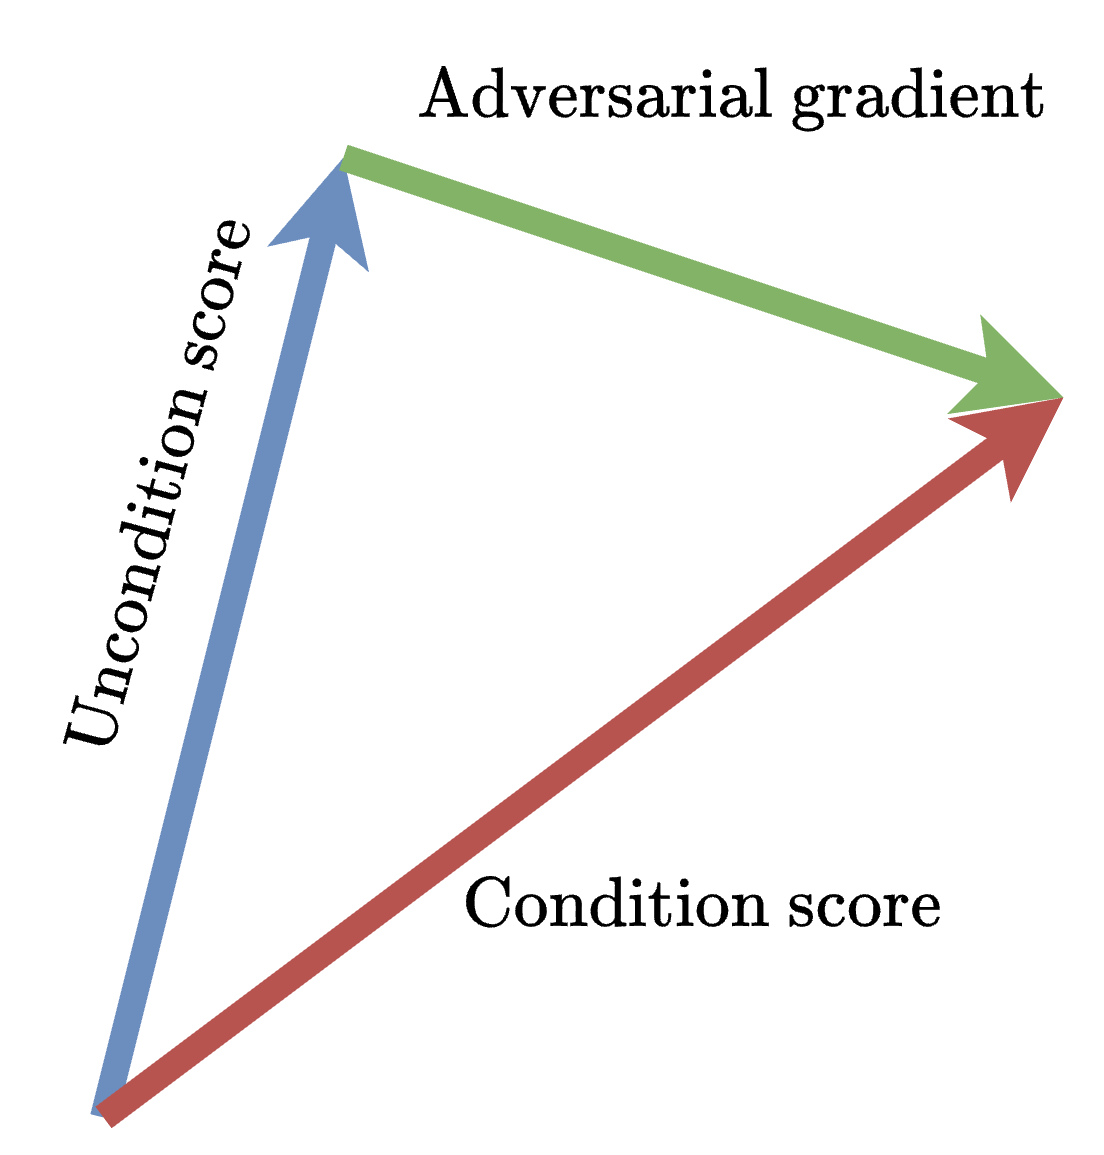
\includegraphics[width=0.7\linewidth]{Vector}
			\end{figure}
%			{\footnotesize
%			\begin{align*}
%				\underbrace{\nabla \log p_{\gamma}(\bx_t | \by)}_{\text{Conditional score}} 
%				&= \underbrace{\nabla \log p(\bx_t)}_{\text{Uncondition score}} + 
%				\underbrace{\gamma \nabla \log p(\by | \bx_t)}_{\text{Adversarial gradient}} \\
%				&= \underbrace{\nabla \log p(\bx_t)}_{\text{Uncondition score}} + 
%				\underbrace{\gamma (\nabla \log p(\bx_t | \by) - \nabla \log p( \bx_t) )}_{\text{Adversarial gradient}} \\
%				&= \underbrace{(1 - \gamma)\nabla \log p(\bx_t)}_{\text{Uncondition score}} + 
%				\underbrace{\gamma \nabla \log p(\bx_t | \by)}_{\text{Condition score}}
%			\end{align*}}
		
		\begin{equation*}
			\hat{\bx}_{0, \gamma, c} = \gamma \cdot f_{\theta} (\bx_t, t, c) + (1-\gamma) \cdot f_{\theta} (\bx_t, t, c_\varnothing)
		\end{equation*}
		
		\vspace{-15pt}
		
	
			
		\end{column}
		
		\begin{column}{0.45\textwidth}
				\begin{figure}
				\centering
				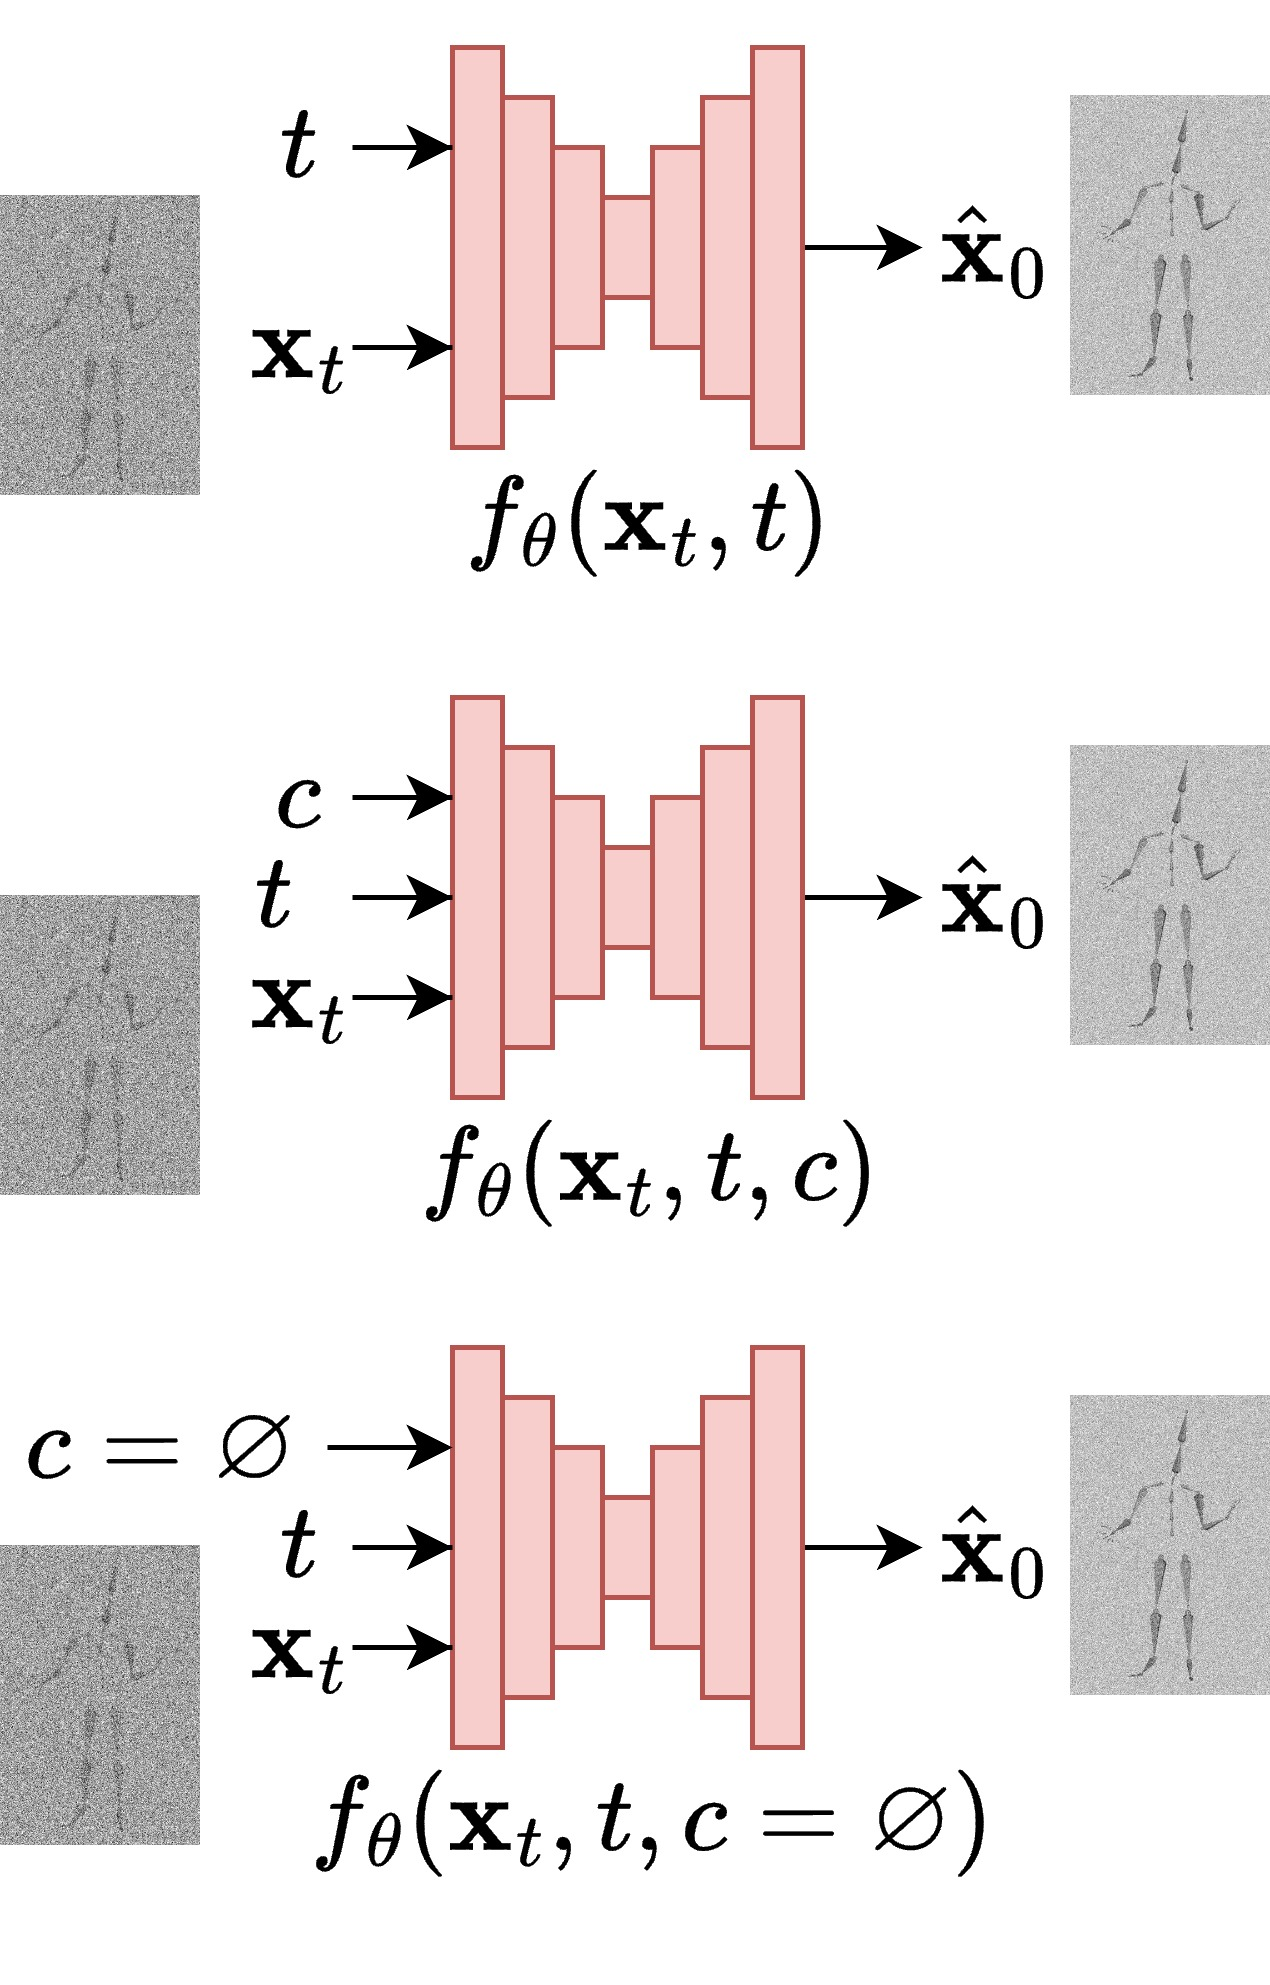
\includegraphics[width=0.9\linewidth]{ConditionDiffusion}
			\end{figure}
		\end{column}
	\end{columns}
	
\end{frame}





